\documentclass{article} % \documentclass{} is the first command in any LaTeX code.  It is used to define what kind of document you are creating such as an article or a book, and begins the document preamble
\usepackage[left=1in, right=1in, top=0.5in, bottom=0.5in]{geometry}
\usepackage{graphicx}
\usepackage{amsmath} % \usepackage is a command that allows you to add functionality to your LaTeX code
\usepackage{subcaption}
\usepackage{ifthen}
\usepackage{xparse}
\usepackage{fancyvrb}
\parindent=0pt % disables indentation

\graphicspath{{../results/}{../writeup/}} 
\newcommand{\img}[3][0.3]{    
    \begin{figure}[h]
        \centering
        \includegraphics[width=\textwidth,keepaspectratio=true,height=#1\textheight]{#2}
        \caption{#3}
    \end{figure}
}
% \newcommand{\subimg}[3][0.5]{    
%     \begin{subfigure}{#1\textwidth}
%         \centering
%         \includegraphics[width=\linewidth,keepaspectratio=true]{#2}
%         \ifthenelse{\equal{#3}{}}{}{\caption{#3}}
%     \end{subfigure}
% }
\NewDocumentCommand{\subimg}{D<>{0.1}mO{}}{    
    \begin{subfigure}{#1\textwidth}
        \centering
        \includegraphics[width=\linewidth,keepaspectratio=true]{#2}
        \ifthenelse{\equal{#3}{}}{}{\caption{#3}}
    \end{subfigure}
}


\title{\large COMP5421 Computer Vision
\\ \huge Homework Assignment 3
\\ \huge Spatial Pyramid Matching for Scene Classification} 
\author{Hartanto Kwee Jeffrey\\
    \normalsize jhk@connect.ust.hk | SID: 20851871} % Sets authors name
\date{}

% The preamble ends with the command \begin{document}
\begin{document} % All begin commands must be paired with an end command somewhere
    \maketitle % creates title using information in preamble (title, author, date)
    
    \section[1]{Representing the World with Visual Words} % creates a section

    \subsection*{1.1 Extracting Filter Responses}
    \subsubsection*{Q1.1.1}

    \begin{enumerate}
        \item Gaussian: in a Gaussian filter, each pixel will store the gaussian-weighted average of its surrounding pixels, so it basically picks up the characteristics of neighbouring pixels. Roughly speaking, each pixel "tells whats happening around it".
        \item Laplacian of Gaussian: edges and corners
        \item derivative of Gaussian in the $x$ direction: vertical edges 
        \item derivative of Gaussian in the $y$ direction: horizontal edges
    \end{enumerate}
    
    We use multiple scales because we want to capture different sizes of surrounding responses to cater for different sizes of features and images. For example, a large sigma may only capture features of neighbours one or two pixels away, while a small sigma may capture wider and large-scale features spanning tens of pixels. For edge detection, larger sigmas are more sensitive to local image gradients and will be more noisy, while smaller sigmas create smoother gradients.

    \subsubsection*{Q1.1.2}
    \img{q1,1.png}{20 filter responses resulting from the filter bank}

    \subsection*{Q1.2}
    This implementation uses $\texttt{alpha} = 200$ and $\texttt{K} = 150$.

    \subsection*{Q1.3}

    Refer to Figure \ref{q13} for the wordmaps.
    \smallskip

    Observing the wordmaps, we see there are clusters of pixels mapped to the same visual word, such as the wooden surfaces of cupboards and white counter top in a kitchen, the ripple pattern of sand in the desert, blue sky with occasional strips of smoky cloud. At the same time, we also see that edges in images are clearly mapped to the same wordmap, showing the effect of the LoG and Sobel Gaussian filters. (If we didn't have these filters and only had Gaussian filters, then these edges may only be mapped different words based on merely its color, and we would see noise instead of the uniform edge colors we see now.) Edges include the counter top and sand ripples. These wordmaps allow images to "speak their features" using visual words, as we see different visual words show up in different frequencies in different images.

    \begin{figure}[h]
        \begin{subfigure}[b]{0.5\textwidth}
            \includegraphics[width=\textwidth]{../data/kitchen/sun_aasmevtpkslccptd.jpg}
        \end{subfigure}
        \begin{subfigure}[b]{0.5\textwidth}
            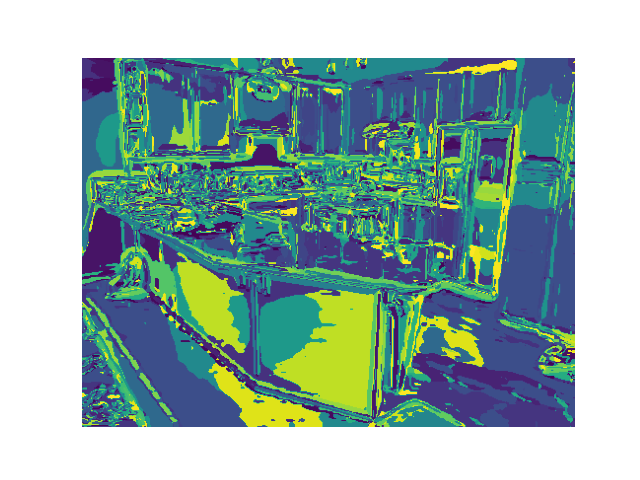
\includegraphics[width=\textwidth]{q1,3_1.png}
        \end{subfigure}
        \begin{subfigure}[b]{0.5\textwidth}
            \includegraphics[width=\textwidth]{../data/desert/sun_aawnvdsxsoudsdwo.jpg}
        \end{subfigure}
        \begin{subfigure}[b]{0.5\textwidth}
            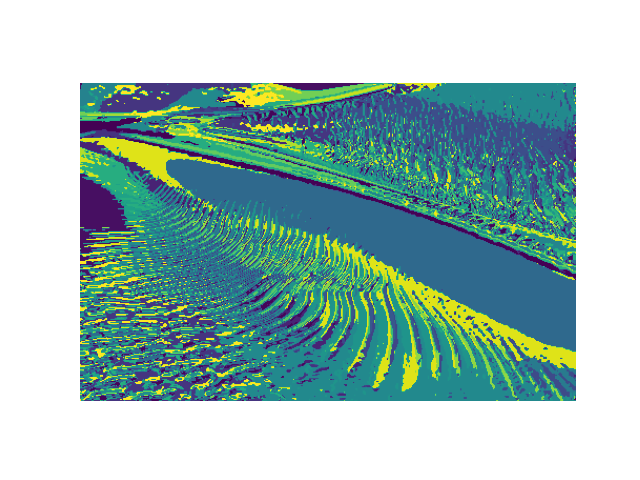
\includegraphics[width=\textwidth]{q1,3_2.png}
        \end{subfigure}
        \begin{subfigure}[b]{0.5\textwidth}
            \includegraphics[width=\textwidth]{../data/highway/sun_acpvugnkzrliaqir.jpg}
        \end{subfigure}
        \begin{subfigure}[b]{0.5\textwidth}
            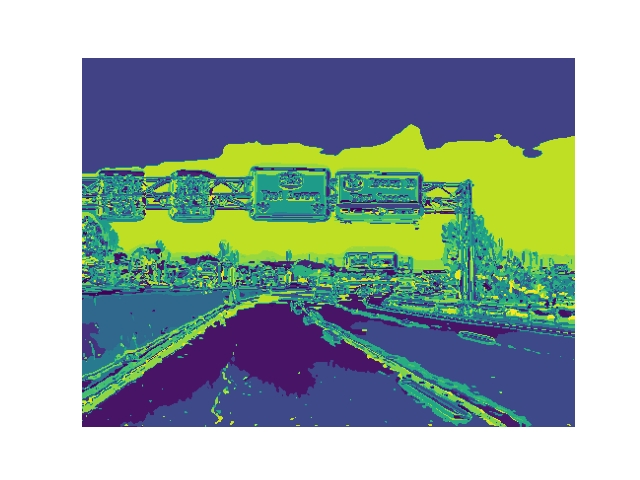
\includegraphics[width=\textwidth]{q1,3_3.png}
        \end{subfigure}
        \begin{subfigure}[b]{0.5\textwidth}
            \includegraphics[width=\textwidth]{../data/waterfall/sun_aecgdxztcovcpyvx.jpg}
        \end{subfigure}
        \begin{subfigure}[b]{0.5\textwidth}
            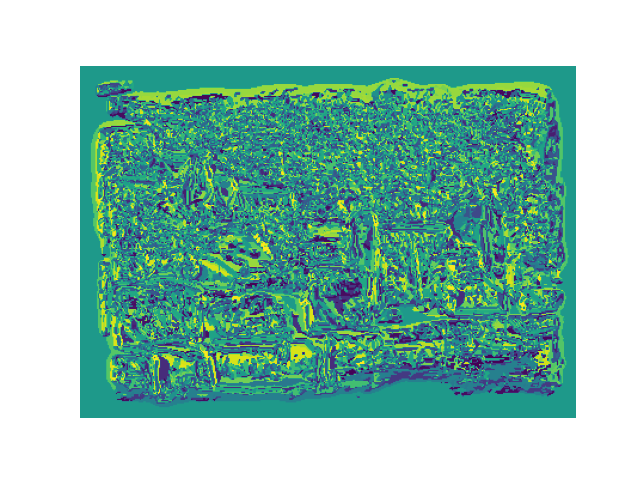
\includegraphics[width=\textwidth]{q1,3_4.png}
        \end{subfigure}
        \caption{Visualized wordmaps of four images.}
        \label{q13}
    \end{figure}
    
    \section[2]{Building a Recognition System}
    \subsection*{Q2.5}

    Confusion matrix:
    \begin{verbatim}   
                                  Predicted Class
                        [[13.  0.  0.  0.  2.  2.  1.  2.]
                         [ 0. 12.  1.  2.  0.  1.  1.  3.]
                         [ 1.  2.  7.  6.  1.  1.  0.  2.]
                  Actual [ 0.  2.  1. 15.  0.  0.  0.  2.]
                   Class [ 3.  0.  1.  0. 11.  3.  0.  2.]
                         [ 1.  0.  0.  1.  8. 10.  0.  0.]
                         [ 2.  0.  0.  0.  0.  2. 16.  0.]
                         [ 0.  1.  0.  5.  0.  0.  0. 14.]]
    \end{verbatim}
    
    Accuracy: 0.6125

    \subsection*{Q2.6}

    Refer to Figure \ref{q26} for the failed cases.
    \smallskip

    If we refer to the confusion matrix, the most frequently misclassified paris are [kitchen, laundromats] (11 cases), [desert, highway] (7 cases) and [highway, windmill] (7 cases).
    \smallskip

    Kitchen and laundromates are both indoor places and share common features such as wooden cupboards, white concrete walls and metallic silver (sinks, oven doors, doors of washing machine etc.).
    \smallskip 
    
    Deserts are frequently misclassified as highways, perhaps because both only consists of a blue sky and a grey concrete road. There are not many edges in highways, so usually large areas of grey are identified as highways. In the two desert images in the failed cases, both have little edge-like features and are predominantly plain gray. This may be the reason why deserts are frequently misidentifed as highways. Conversely, highways are not frequently missclassfied perhaps because of the presence of road signs.
    \smallskip

    Highways are frequently misclassified as windmills. In the three failed cases shown, there are roads in addition to the windmills. Since the windmill only takes up a small area in the image, the effect of the road-like features dominate the prediction, and causes these images to be misclassified as highways.

    \begin{figure}[h]
        \begin{subfigure}[b]{0.333\textwidth}
            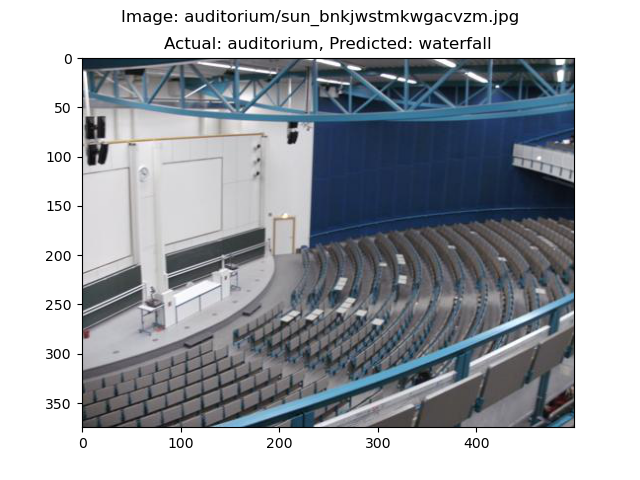
\includegraphics[width=\textwidth]{q2,6_case_10.png}
        \end{subfigure}
        \begin{subfigure}[b]{0.333\textwidth}
            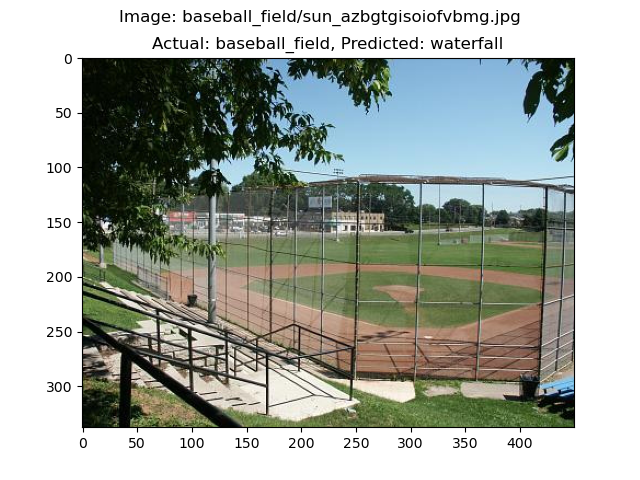
\includegraphics[width=\textwidth]{q2,6_case_22.png}
        \end{subfigure}
        \begin{subfigure}[b]{0.333\textwidth}
            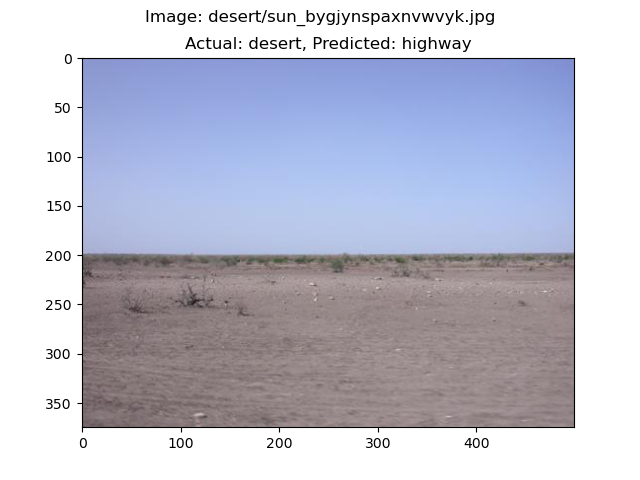
\includegraphics[width=\textwidth]{q2,6_case_49.png}
        \end{subfigure}
        \begin{subfigure}[b]{0.333\textwidth}
            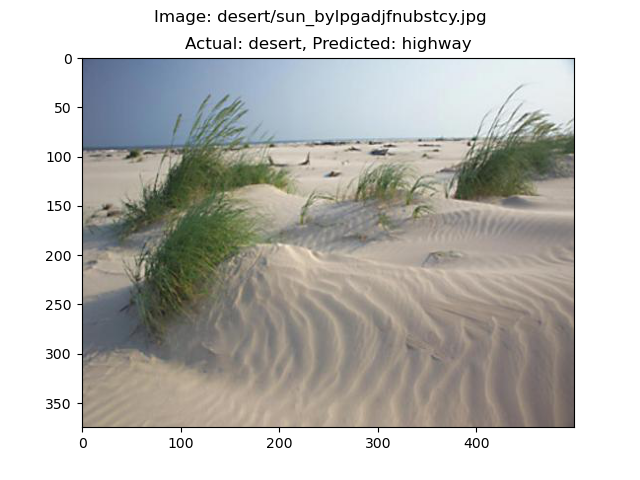
\includegraphics[width=\textwidth]{q2,6_case_51.png}
        \end{subfigure}
        \begin{subfigure}[b]{0.333\textwidth}
            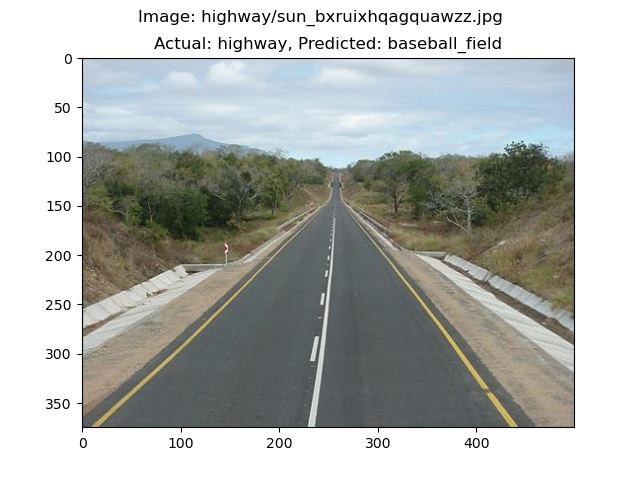
\includegraphics[width=\textwidth]{q2,6_case_68.png}
        \end{subfigure}
        \begin{subfigure}[b]{0.333\textwidth}
            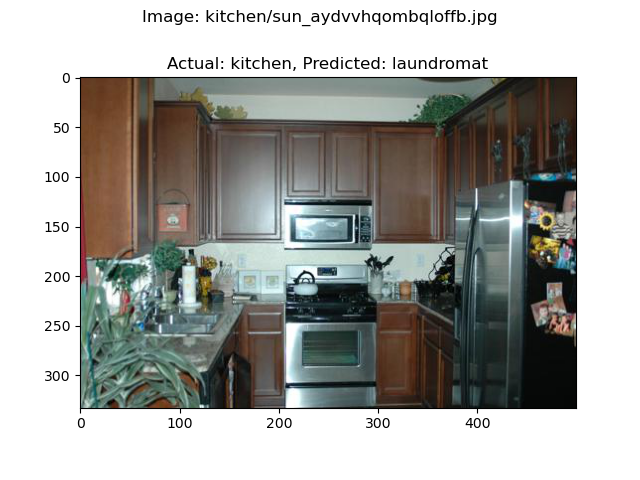
\includegraphics[width=\textwidth]{q2,6_case_88.png}
        \end{subfigure}
        \begin{subfigure}[b]{0.333\textwidth}
            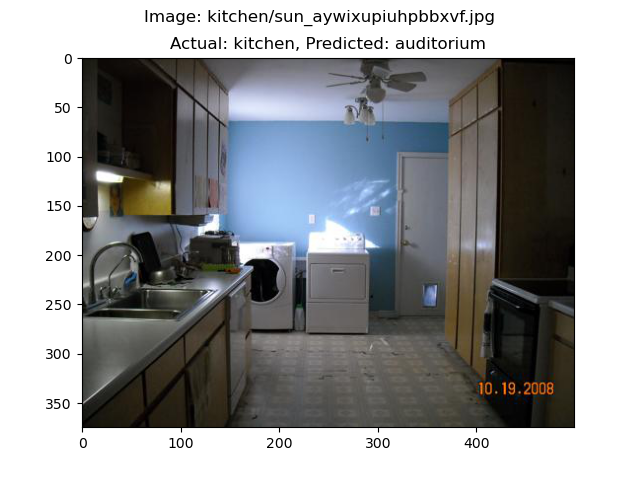
\includegraphics[width=\textwidth]{q2,6_case_91.png}
        \end{subfigure}
        \begin{subfigure}[b]{0.333\textwidth}
            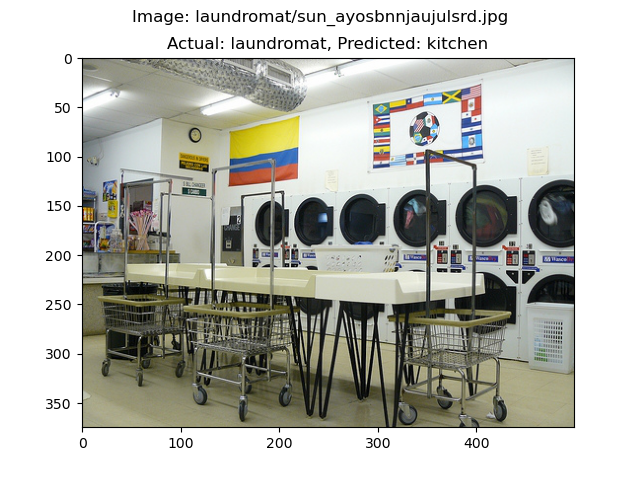
\includegraphics[width=\textwidth]{q2,6_case_107.png}
        \end{subfigure}
        \begin{subfigure}[b]{0.333\textwidth}
            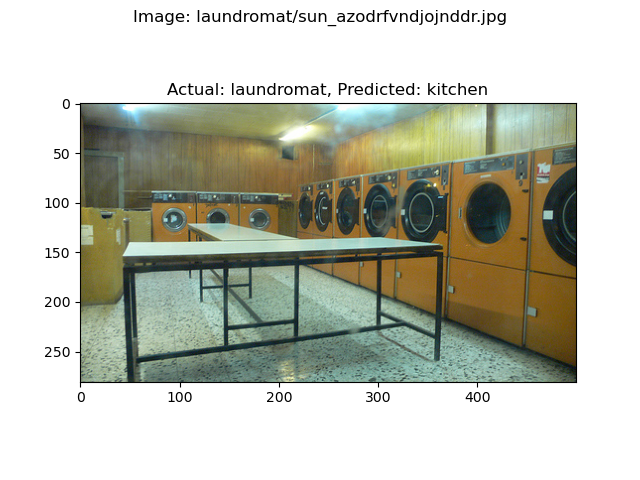
\includegraphics[width=\textwidth]{q2,6_case_117.png}
        \end{subfigure}
        \begin{subfigure}[b]{0.333\textwidth}
            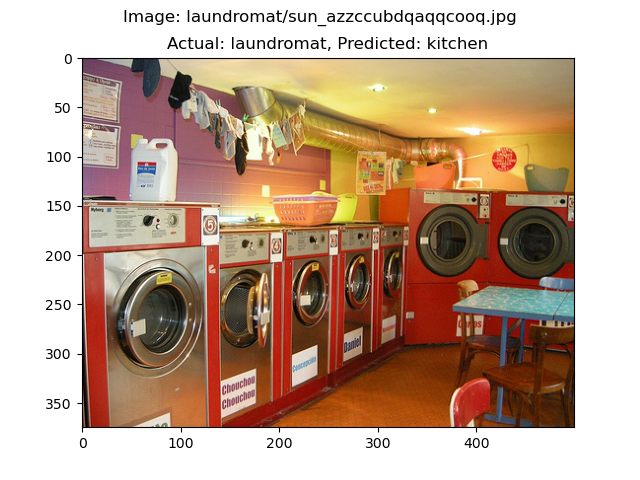
\includegraphics[width=\textwidth]{q2,6_case_119.png}
        \end{subfigure}
        \begin{subfigure}[b]{0.333\textwidth}
            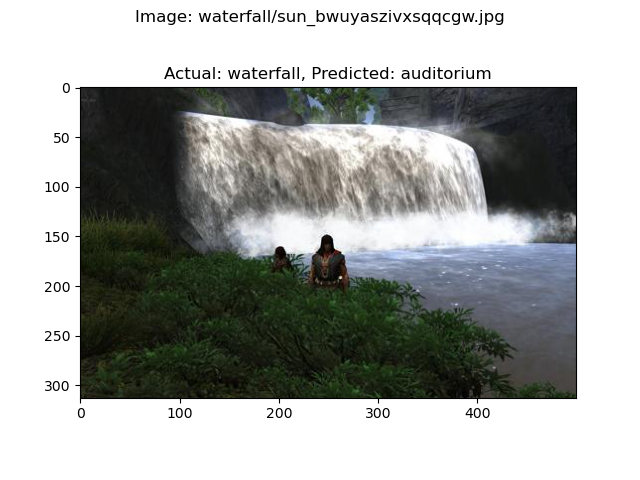
\includegraphics[width=\textwidth]{q2,6_case_131.png}
        \end{subfigure}
        \begin{subfigure}[b]{0.333\textwidth}
            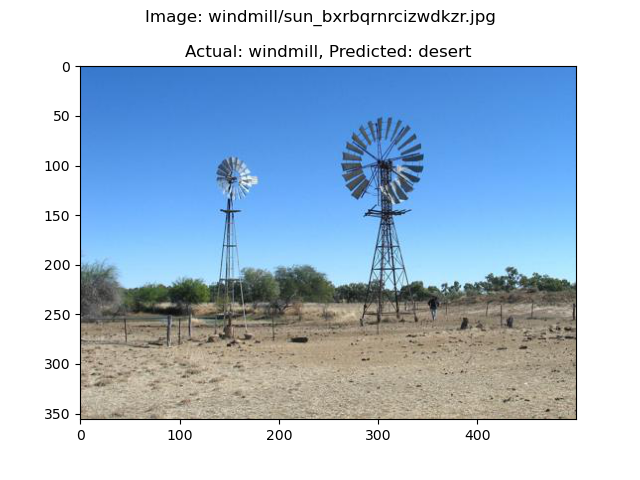
\includegraphics[width=\textwidth]{q2,6_case_144.png}
        \end{subfigure}
        \begin{subfigure}[b]{0.333\textwidth}
            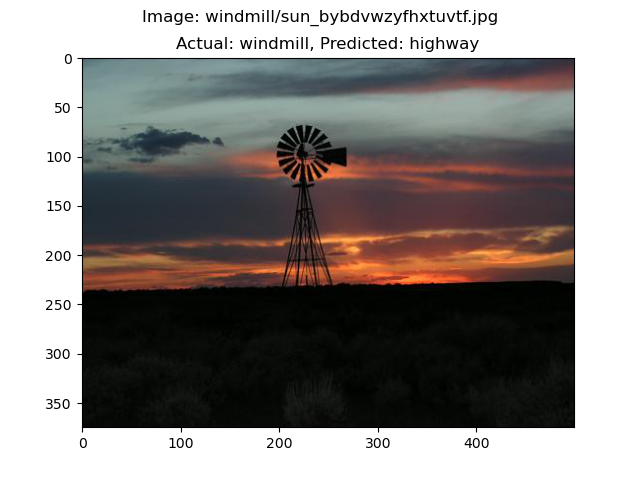
\includegraphics[width=\textwidth]{q2,6_case_147.png}
        \end{subfigure}
        \begin{subfigure}[b]{0.333\textwidth}
            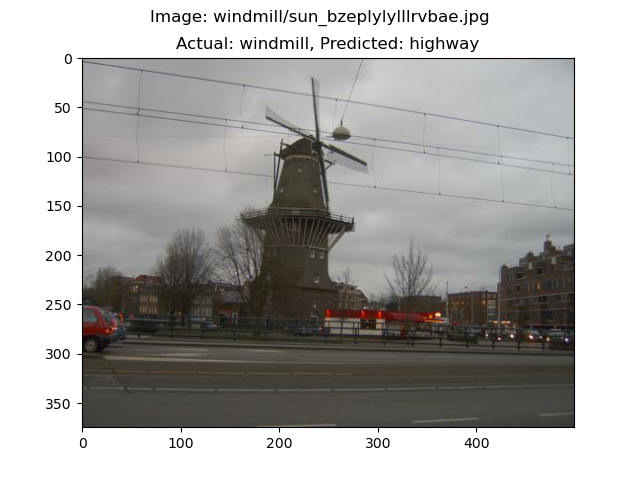
\includegraphics[width=\textwidth]{q2,6_case_154.png}
        \end{subfigure}
        \begin{subfigure}[b]{0.333\textwidth}
            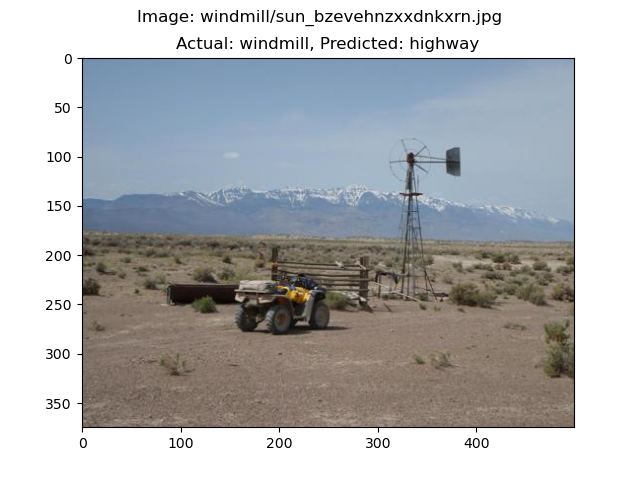
\includegraphics[width=\textwidth]{q2,6_case_156.png}
        \end{subfigure}
        \caption{Failed cases with their predicted and actual class.}
        \label{q26}
    \end{figure}

    \section[3]{Deep Learning Features}
    \subsection*{Q3.2}
    Confusion matrix:
    \begin{Verbatim}[samepage=true]
                                  Predicted Class
                        [[19.  0.  0.  0.  1.  0.  0.  0.]
                         [ 1. 16.  1.  0.  0.  0.  1.  1.]
                         [ 0.  0. 19.  1.  0.  0.  0.  0.]
                  Actual [ 0.  0.  0. 20.  0.  0.  0.  0.]
                   Class [ 0.  0.  0.  0. 19.  1.  0.  0.]
                         [ 0.  0.  0.  0.  1. 19.  0.  0.]
                         [ 0.  0.  1.  0.  0.  0. 19.  0.]
                         [ 0.  0.  0.  1.  0.  0.  0. 19.]]
    \end{Verbatim}

    Accuracy: 0.9375
    \smallskip

    The accuracy of deep features is much higher than bag of words.
    \smallskip

    In our discussion of the bag of words failed cases, we observe that a lot of misclassification stems from sharing features with other classes. If the unique feature of the actual class takes only a small area, our histogram-based matching would easily neglect this feature and misclassify.
    \smallskip

    Deep features are more robust as they capture both wide-scale and small-scale features, and places different weighting on these features as opposed to histogram matching. Therefore, unique features may lead to greater activations and dominate the network output.

\end{document} % This is the end of the document